



\lstset{language=R}
\begin{lstlisting}
library(colorspace)
library(classInt)
library(sp)
library(maptools)
library(rgdal)

airStations <- read.csv2('data/airStations.csv')
coordinates(airStations) <- ~ long + lat
proj4string(airStations) <- CRS("+proj=longlat +ellps=WGS84")

airQuality <- read.csv2('data/airQuality.csv')

NO2 <- airQuality[airQuality$codParam==8, ]
NO2mean <- aggregate(dat ~ codEst, NO2, FUN=mean)
idxNO2 <- match(airStations$Codigo, NO2mean$codEst)
airStations$NO2 <- NO2mean$dat[idxNO2]
\end{lstlisting}


\lstset{language=R}
\begin{lstlisting}
obj <- airStations['NO2']
xy <- xy.coords(coordinates(obj))
z <- stack(obj)

intervals <- classIntervals(z$values, n=4, style='fisher')
nInt <- length(intervals$brks) - 1

idx <- findCols(intervals)
size <- c(0.6, 1.5)
rval <- seq(1, 0, length=nInt)
pwr.size <- 0.8
cex.key <- size[2] - diff(size)*rval^pwr.size 
cex <- cex.key[idx]

pal <- rev(heat.ob(n=nInt, beg=1, end=200))
col <- findColours(intervals, pal)
col.key=attr(col, 'palette')


tabInt <- getFromNamespace('tableClassIntervals', 'classInt')
op <- options(digits=2)
tab <- tabInt(cols = idx, brks = intervals$brks,
              under = "under", over = "over", between = "-", 
              cutlabels = TRUE,
              intervalClosure = "left",
              dataPrecision = NULL)
options(op)

key <- list(x = 0.02, y = 0.02, corner = c(0, 0),
            title=expression(NO[2]~~(paste(mu, plain(g))/m^3)),
            cex.title=.75,
            background='gray90', 
            text=list(labels=names(tab), cex=0.85),
            points=list(col=col.key, pch=19, cex=cex.key))
\end{lstlisting}


\lstset{language=R}
\begin{lstlisting}
longlatScales <- getFromNamespace('longlat.scales', 'sp')
bbExpand <- getFromNamespace('bbexpand', 'sp')
scales <- longlatScales(obj,
                        scales=list(draw = TRUE, cex=0.7),
                        xlim = bbExpand(bbox(obj)[1, ], 0.2),
                        ylim = bbExpand(bbox(obj)[2, ], 0.1))
\end{lstlisting}

\lstset{language=R}
\begin{lstlisting}
panel.bubbles <- function(x, y, subscripts, col, radius,...){
  colors <- col[subscripts]
  radius <- unit(.05*radius[subscripts], 'inch')

  grid.circle(x, y, radius,
              default.units='native',
              gp=gpar(col=colors,
                fill=adjustcolor(colors, alpha=.85),
                lwd=1, ...)
              )
    }
\end{lstlisting}


\lstset{language=R}
\begin{lstlisting}
p <- xyplot(lat ~ long, data=z,
            xlab='', ylab='', main='',
            cex=cex, col=col, radius=cex,
            key=key, 
            asp=mapasp(obj), scales=scales,
            panel=panel.bubbles)
\end{lstlisting}


\lstset{language=R}
\begin{lstlisting}
## nomecalles http://www.madrid.org/nomecalles/Callejero_madrid.icm
## Form at http://www.madrid.org/nomecalles/DescargaBDTCorte.icm

## Distritos de Madrid
unzip('Distritos de Madrid.zip')
distritosMadrid <- readShapePoly('Distritos de Madrid/200001331')
proj4string(distritosMadrid) <- CRS("+proj=utm +zone=30")
distritosMadrid <- spTransform(distritosMadrid, CRS=CRS("+proj=longlat +ellps=WGS84"))

## Callejero: Ejes de viales
unzip('Callejero_ Ejes de viales.zip')
streets <- readShapeLines('Callejero_ Ejes de viales/call2011.shp')
streetsMadrid <- streets[streets$CMUN=='079',]
proj4string(streetsMadrid) <- CRS("+proj=utm +zone=30")
streetsMadrid <- spTransform(streetsMadrid, CRS=CRS("+proj=longlat +ellps=WGS84"))
\end{lstlisting}




\lstset{language=R}
\begin{lstlisting}
p +
  layer_(sp.polygons(distritosMadrid, fill='gray92', lwd=0.3)) +
  layer(sp.lines(streetsMadrid, lwd=0.05)) +
  layer(sp.pointLabel(airStations, labels=airStations$Nombre,
                      cex=0.6, fontfamily='Palatino'))
\end{lstlisting}

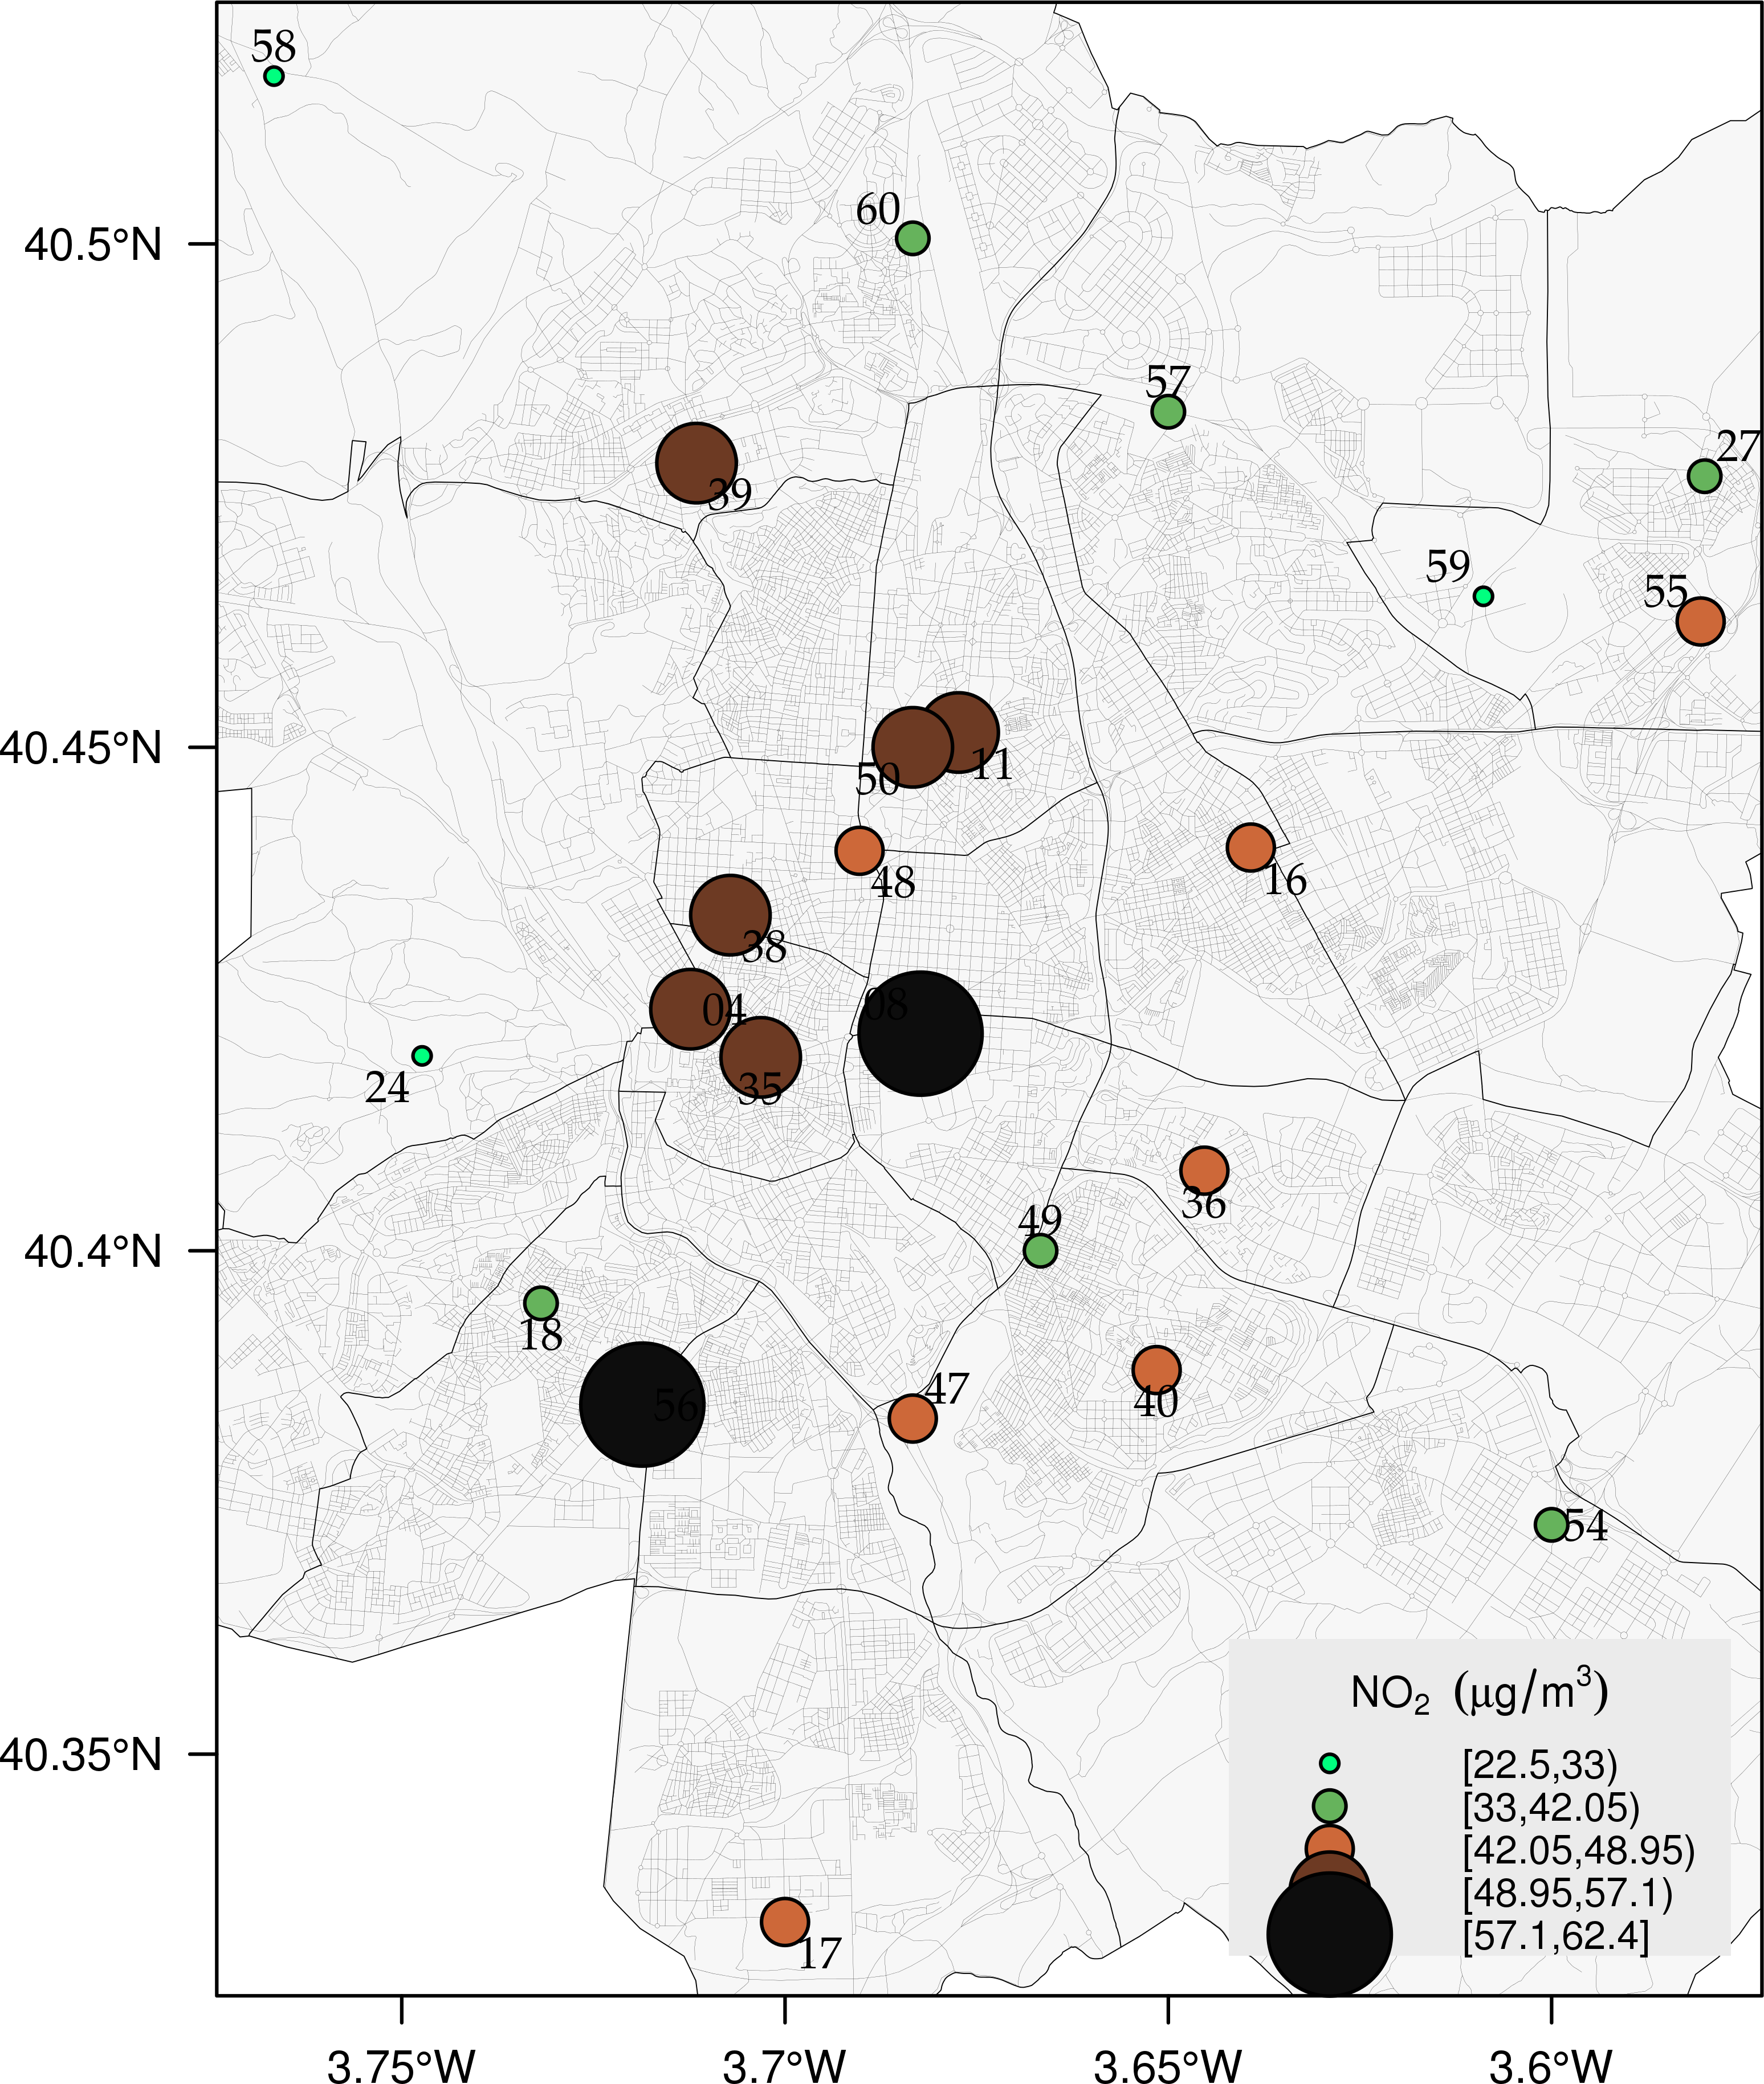
\includegraphics[width=.9\linewidth]{figs/airMadrid.pdf}

